\documentclass[14pt]{extreport}
\usepackage{gost}

\begin{document}

\pagestyle{empty}

\includepdf{titulCourse.pdf}
\pagestyle{plain}

\tableofcontents

\chapter{Введение}

\section{Задание}

Создать программное обеспечение системы обработки данных: «Программа для контроля собственных денежных средств».

Необходимо реализовать следующие функции, позволяющие:
\begin{enumerate}
\item Добавлять продукт в коллекцию (тип коллекции на ваш выбор).
\item Просматривать все записанное в программу.
\item Просматривать покупки по дате и категории.
\item Распределять их по стоимости от минимальной к максимальной или наоборот.
\item Удалять требуемые записи и выходить из программы.
\end{enumerate}

Дополнительные указания: интерфейс программы реализовать в отдельной функции на ваше усмотрение.

Рекомендуется реализовать возможность сохранения данных в файл.

\section{Цель работы}

Создать программное обеспечение системы обработки данных в виде интерактивного консольного приложения в Python3: «Программа для
контроля собственных денежных средств».

\section{Задачи}

\begin{enumerate}
\item Описать этапы анализа предметной области и требований
\item Описать решение задания с указанием применения элементов программирования
\item Представить графические материалы, блок-схемы алгоритмов
\item Графически продемонстрировать работу информационной системы
\end{enumerate}

\chapter{Ход работы}

\section{Анализ предметной области и требований}

Система предназначена для учета собственных денежных средств и для повышения финансовой грамотности пользователя. Программа напоминает мобильные приложения банков, где используют системы контроля денежных средств, которые предоставляются клиентам банка. 

Требуется, чтобы приложение:
\begin{enumerate}
\item имело интуитивно-понятный интерфейс,
\item имело функции добавления/удаления продукта,
\item умело отображать все продукты или в соответствии с датой/категорией,
\item умело сортировать продукты по стоимости,
\item умело обрабатывать некорректно введёные значения, любые действия пользователя,
\item умело сохранять данные о продуктах в коллекции.
\end{enumerate}

Взаимодействие с пользователем должно происходить в режиме реального времени, то есть, если пользователь делает запрос к системе, то получает ответ по завершении обработки процесса в программе.

Все продукты, которые пользователь захочет сохранить в коллекции по завершении работы программы, будут хранится в текстовом файле, из которого программа извлекает данные после запуска.

Проектирование интеллектуальной системы будет реализовано на высокоуровневом языке программирования Python3, который имеет достаточно эффективности и функционала, чтобы реализовать программу, соответствующую требованиям. Взаимодействие с пользователем будет происходить в интерактивной командной строке.

\section{Реализация программы}

В начале программы реализовано приветствие пользователя (рис. \ref{fig11}, \ref{fig14}).

\begin{figure}[H]
\centerline{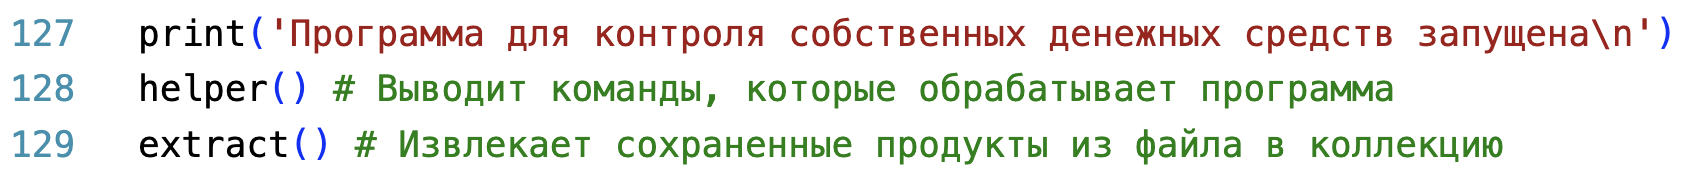
\includegraphics[width=1\linewidth]{Pic1.png}}
\caption{Код приветствия пользователя}
\label{fig11}
\end{figure}

Функция helper() выводит команды, которые распознаёт программа (рис. \ref{fig12}). 

\begin{figure}[H]
\centerline{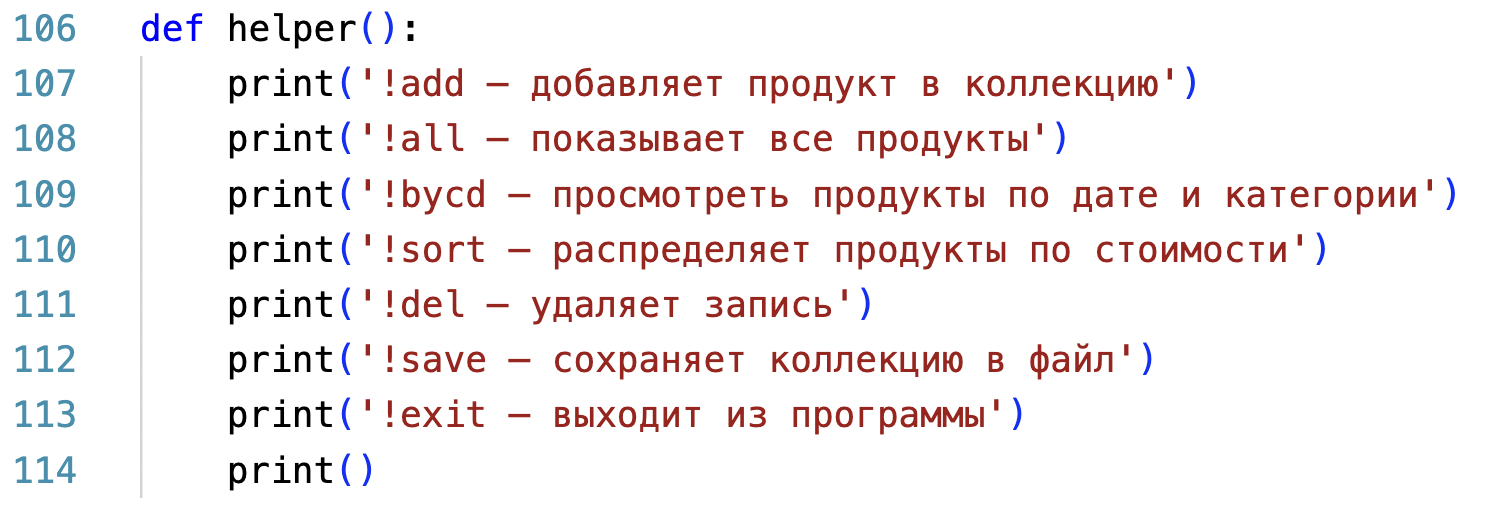
\includegraphics[width=1\linewidth]{Pic2.png}}
\caption{Код функции helper()}
\label{fig12}
\end{figure}

Функция extract() извлекает из текстового файла все имеющиеся записи с прошлых сессий работы программы и добавляет в коллекцию (рис. \ref{fig13}). 

\begin{figure}[H]
\centerline{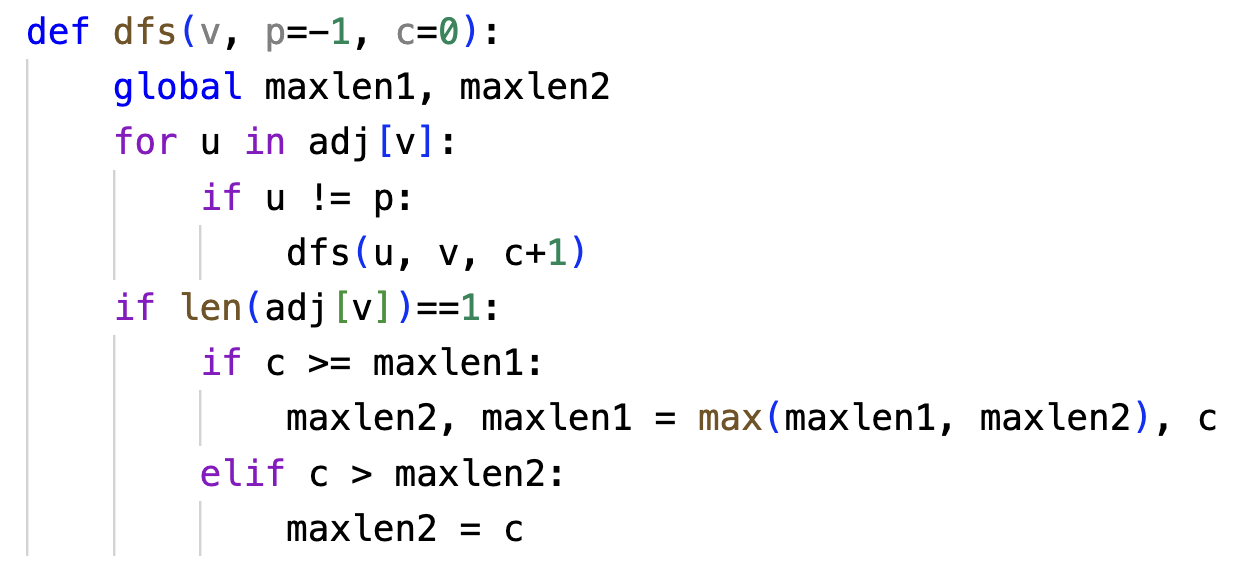
\includegraphics[width=1\linewidth]{Pic3.png}}
\caption{Код функции extract()}
\label{fig13}
\end{figure}

\begin{figure}[H]
\centerline{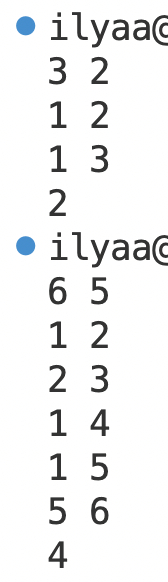
\includegraphics[width=1\linewidth]{Pic4.png}}
\caption{Вывод приветствия в консоли}
\label{fig14}
\end{figure}

Далее запускается бесконечный цикл, в котором пользователь взаимодействует с системой, посредством набора команд (рис. \ref{fig15}). В бесконечном цикле, программа требует ввести команду для выполнения, чтобы запустить соответствующую этой команде функцию. Пример корректной команды: рис. \ref{fig16}. Примеры набора некорректных команд: рис. \ref{fig17}.

\begin{figure}[H]
\centerline{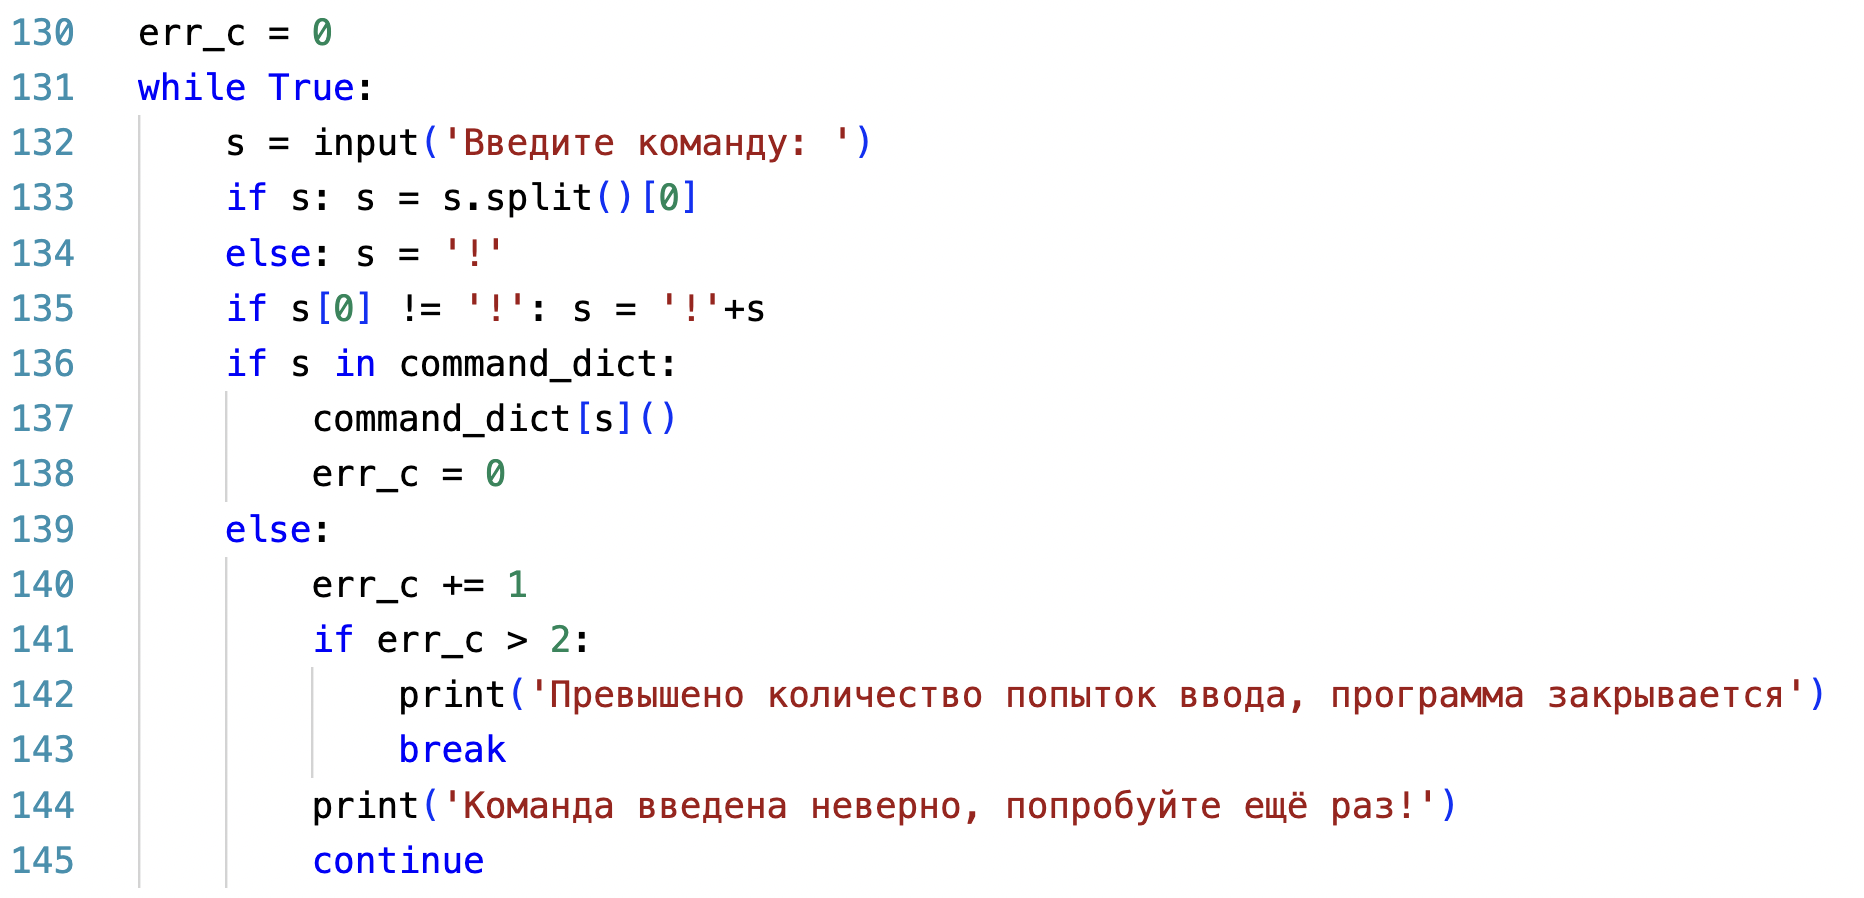
\includegraphics[width=1\linewidth]{Pic5.png}}
\caption{Бесконечный цикл, в котором вводятся команды}
\label{fig15}
\end{figure}

\begin{figure}[H]
\centerline{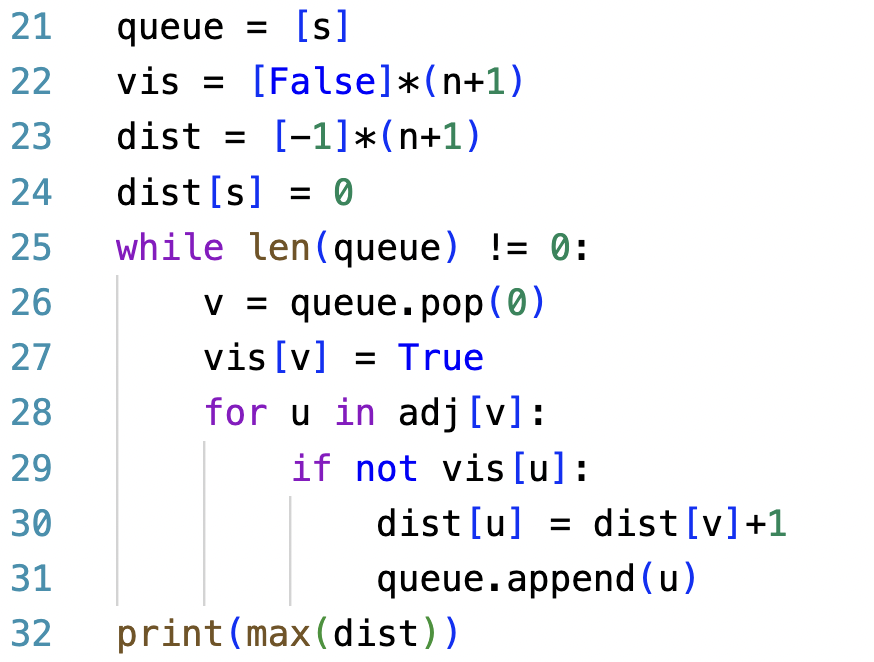
\includegraphics[width=1\linewidth]{Pic6.png}}
\caption{Пример ввода команды all для вывода всех записей}
\label{fig16}
\end{figure}

\begin{figure}[H]
\centerline{
\includegraphics[width=1\linewidth]{Pic7.png}}
\caption{Пример обработки неверных команд}
\label{fig17}
\end{figure}

\begin{figure}[H]
\centerline{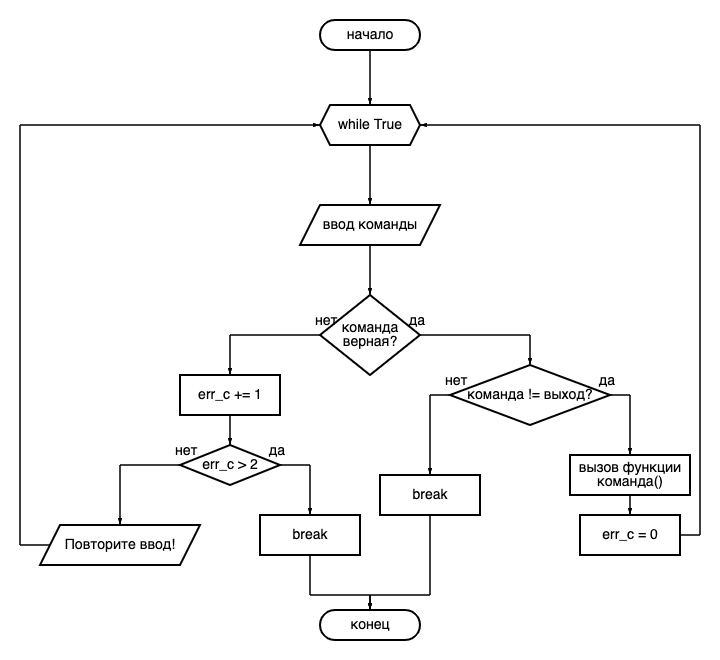
\includegraphics[width=1\linewidth]{diagram1.png}}
\caption{Блок-схема кода с бесконечным циклом}
\end{figure}

Все взаимодействие, что может выполнять программа реализовано в отдельных функциях, которые вызываются при вводе соответствующей им команды. Рассмотрим функции по порядку.

Функция add() для добавления продукта в коллекцию (рис. \ref{fig18}) при вызове требует ввести название продукта, категорию, стоимость, дату покупки (рис. \ref{fig19}).
Функция add() добавляет продукт в двумерный список collection, который хранит все данные о покупках.

\begin{figure}[H]
\centerline{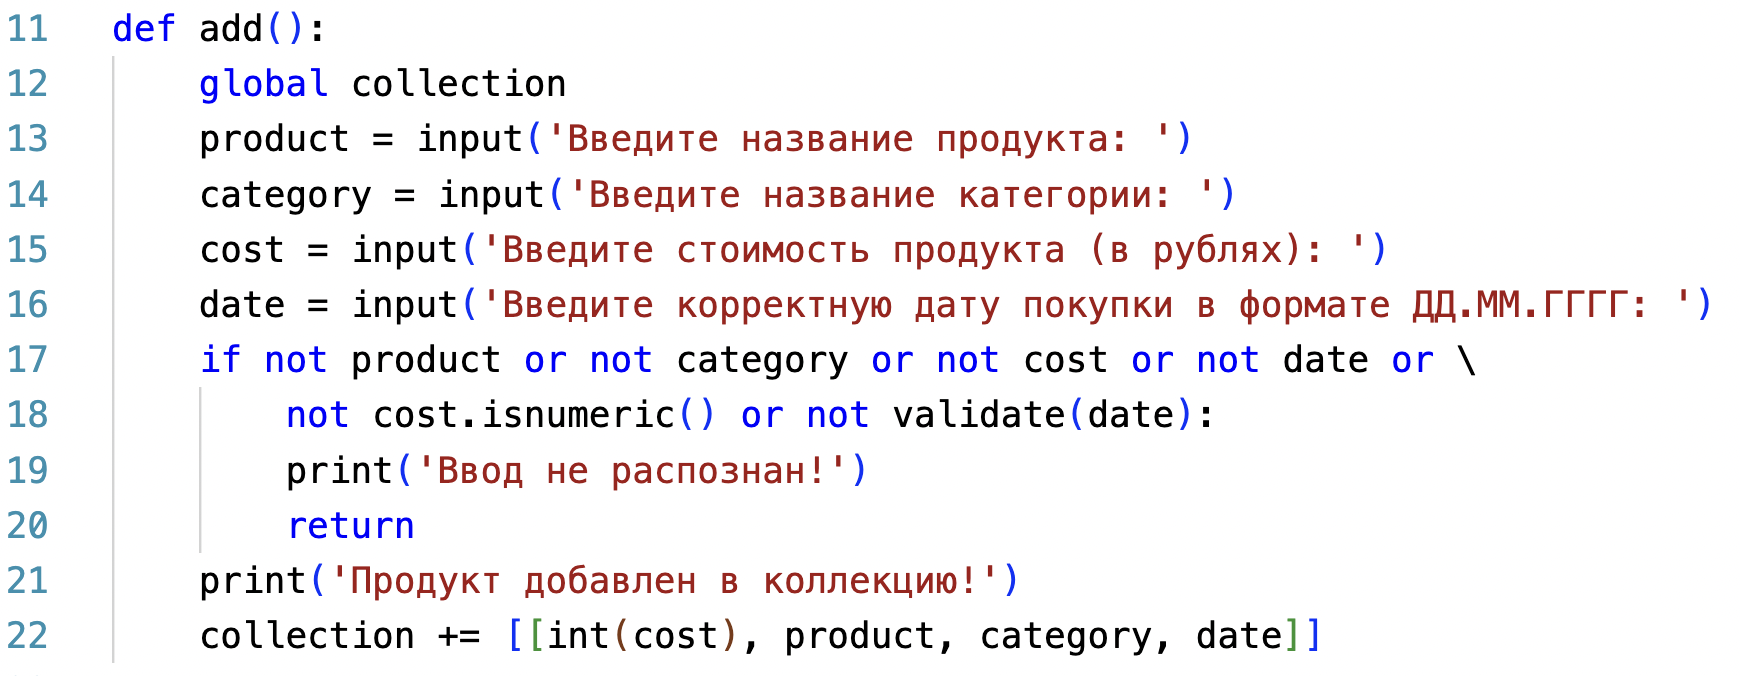
\includegraphics[width=1\linewidth]{Pic8.png}}
\caption{Код функции add()}
\label{fig18}
\end{figure}

\begin{figure}[H]
\centerline{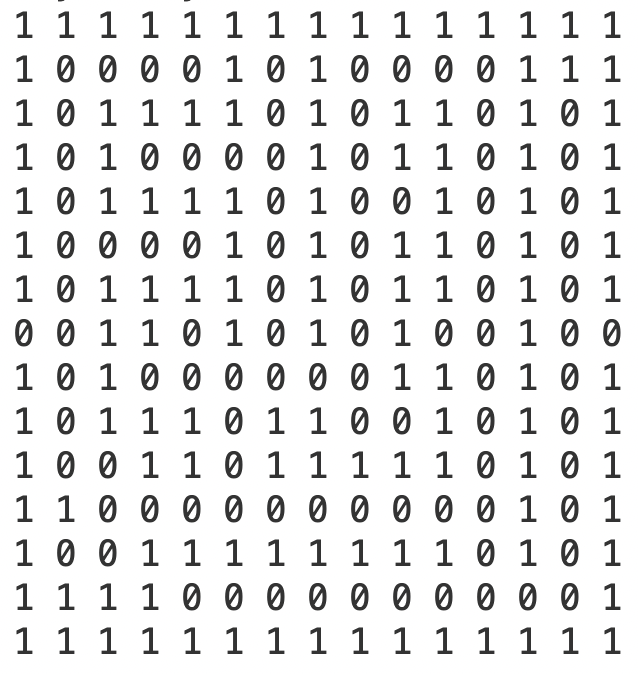
\includegraphics[width=1\linewidth]{Pic9.png}}
\caption{Пример работы команды add}
\label{fig19}
\end{figure}

\begin{figure}[H]
\centerline{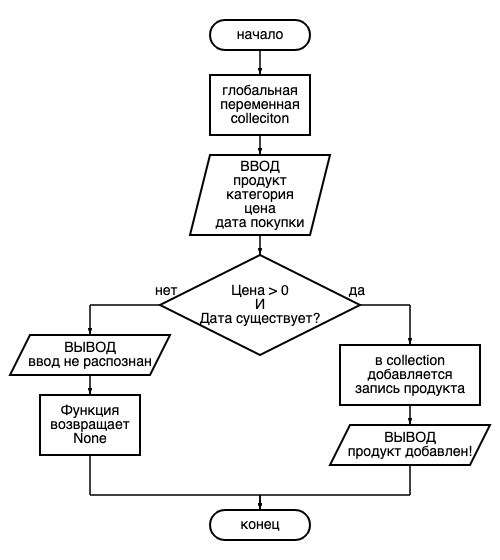
\includegraphics[width=1\linewidth]{diagram2.png}}
\caption{Блок-схема функции add()}
\end{figure}

Функция All() для просмотра всех добавленных в коллекцию продуктов (рис. \ref{fig20}). 
Данная функция выводит все продукты, которые хранятся в двумерном списке collection.
Для красивого вывода в виде таблицы (рис. \ref{fig21}) используются вспомогательные функции table\_title() и table\_item() (рис.\ref{fig22}, \ref{fig23}). 

\begin{figure}[H]
\centerline{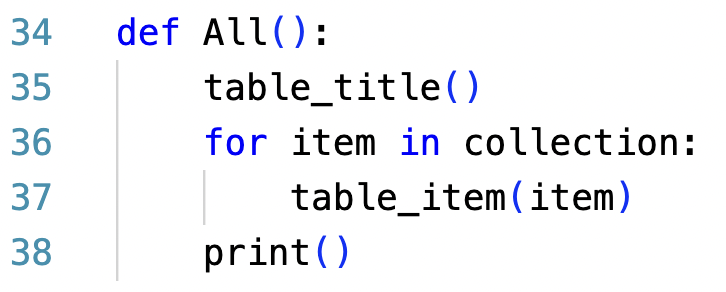
\includegraphics[width=0.4\linewidth]{Pic10.png}}
\caption{Код функции All()}
\label{fig20}
\end{figure}

\begin{figure}[H]
\centerline{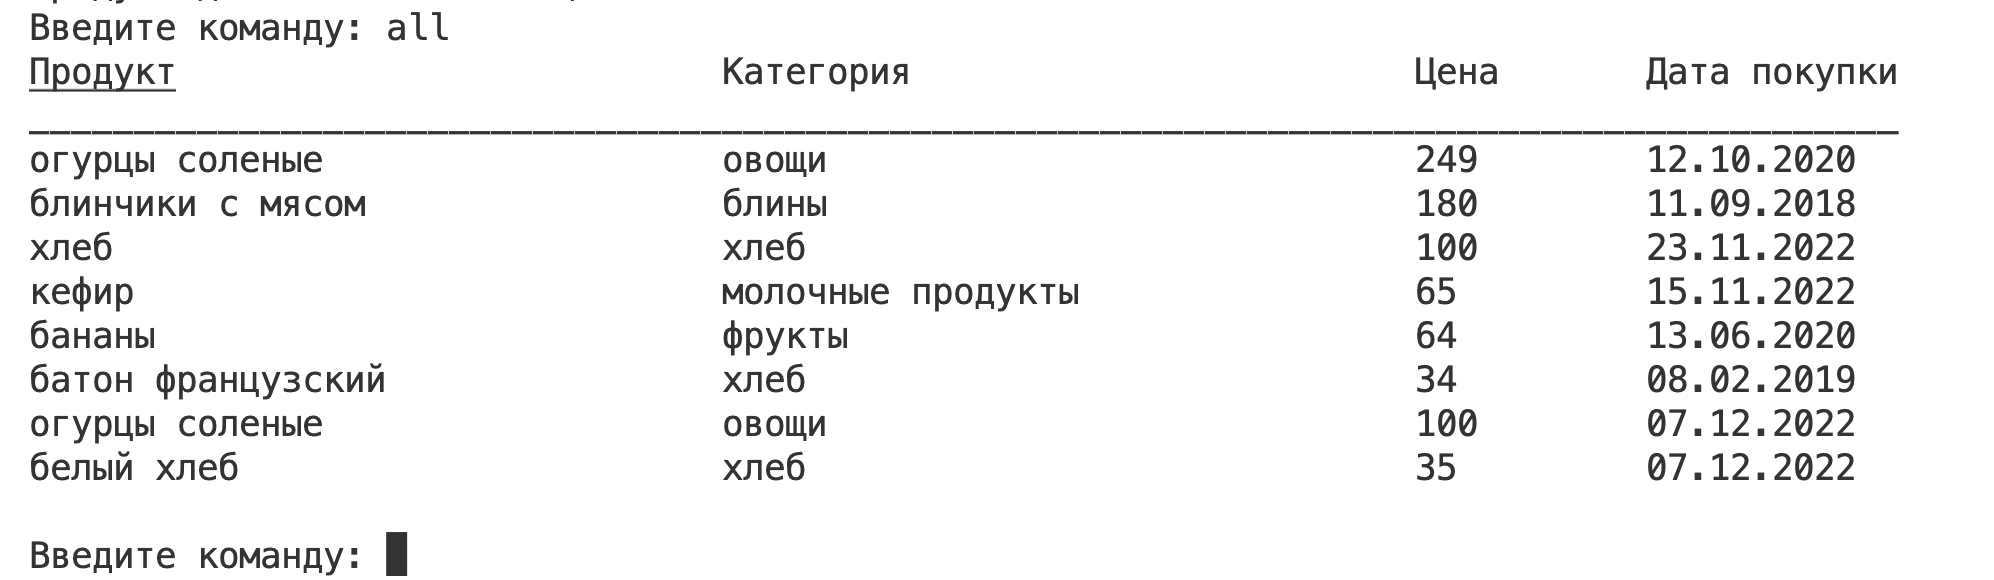
\includegraphics[width=1\linewidth]{Pic11.png}}
\caption{Пример работы команды all}
\label{fig21}
\end{figure}

\begin{figure}[H]
\centerline{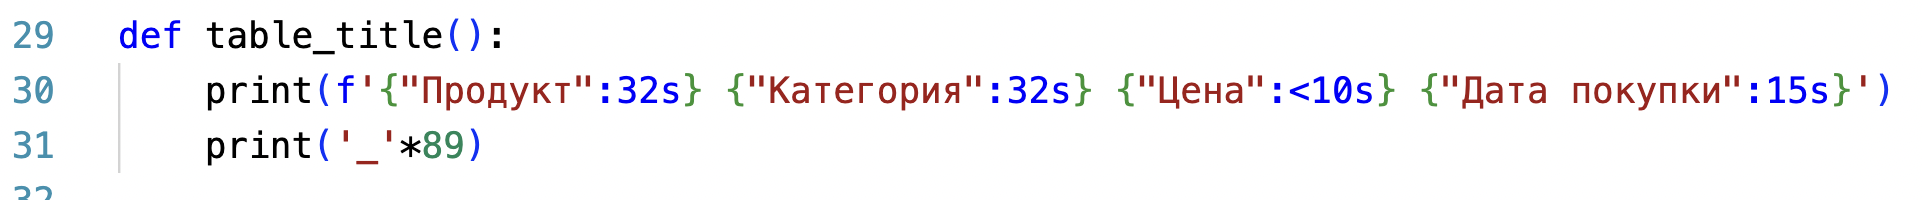
\includegraphics[width=1\linewidth]{Pic12.png}}
\caption{Код функции table\_title()}
\label{fig22}
\end{figure}

\begin{figure}[H]
\centerline{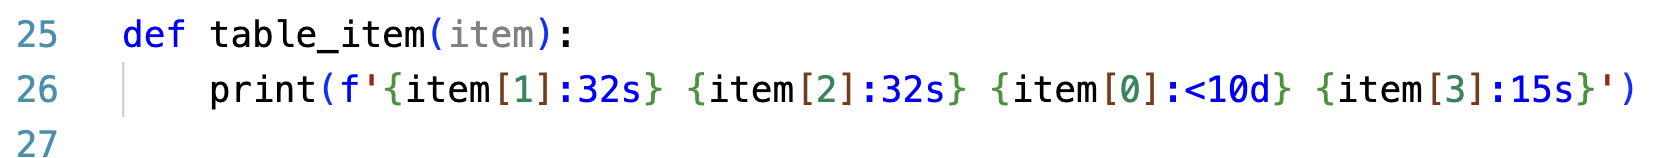
\includegraphics[width=1\linewidth]{Pic13.png}}
\caption{Код функции table\_item()}
\label{fig23}
\end{figure}

Функция bycd() для просмотра продуктов по дате или категории (рис. \ref{fig24}). Данная функция требует от пользователя ввода названия категории или даты и выводит все записи в коллекции, которые имеют ту же дату или категорию (рис. \ref{fig25}, \ref{fig26}). Если в коллекции отсутствуют соответствующие продукты, то выводится таблица без продуктов (рис. \ref{fig27}).

\begin{figure}[H]
\centerline{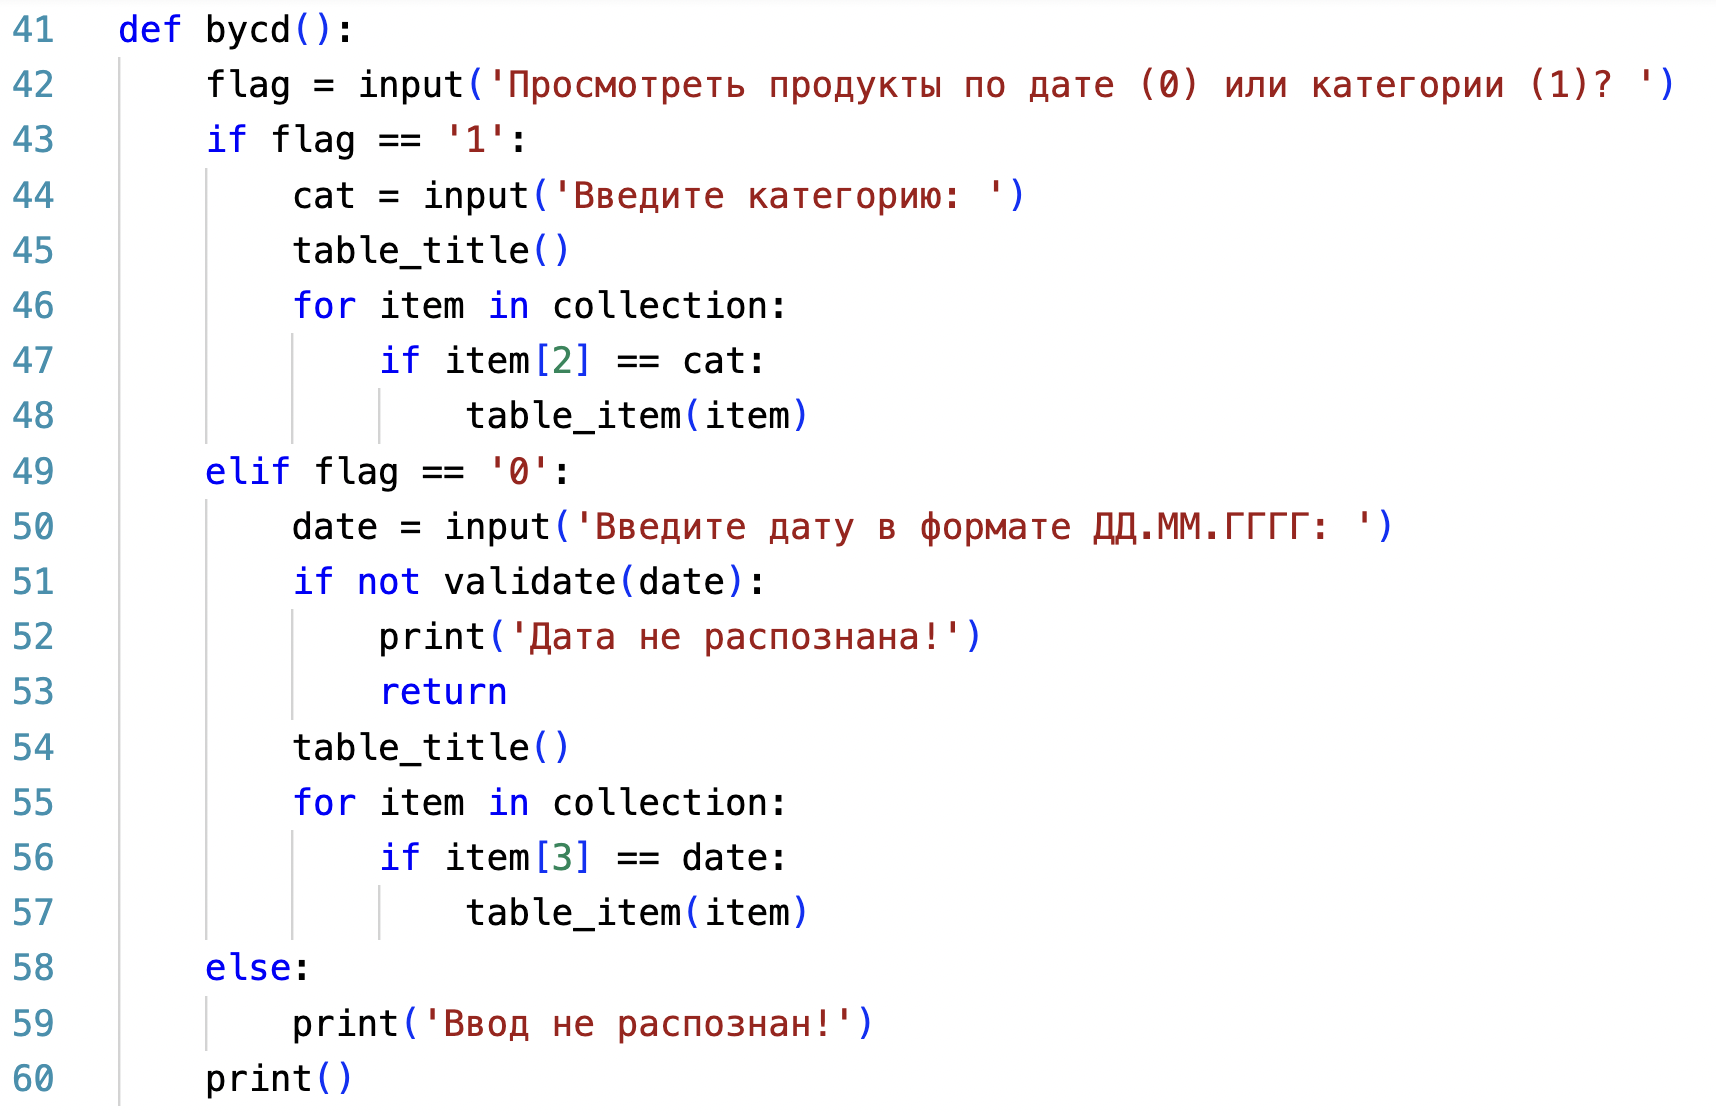
\includegraphics[width=1\linewidth]{Pic14.png}}
\caption{Код функции bycd()}
\label{fig24}
\end{figure}

\begin{figure}[H]
\centerline{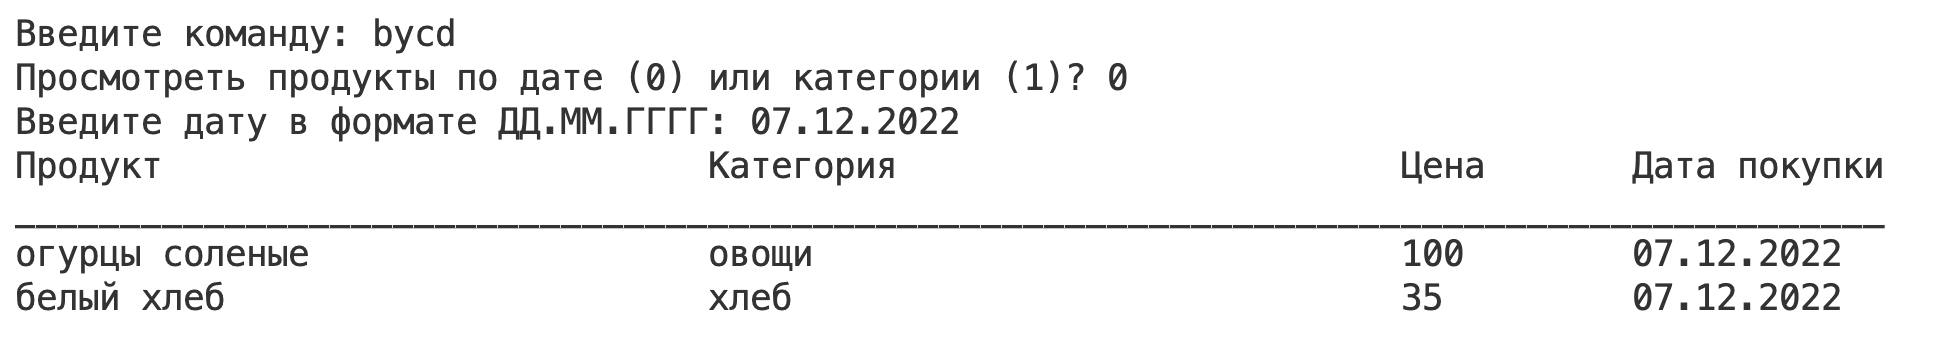
\includegraphics[width=1\linewidth]{Pic15.png}}
\caption{Пример работы команды bycd по дате}
\label{fig25}
\end{figure}

\begin{figure}[H]
\centerline{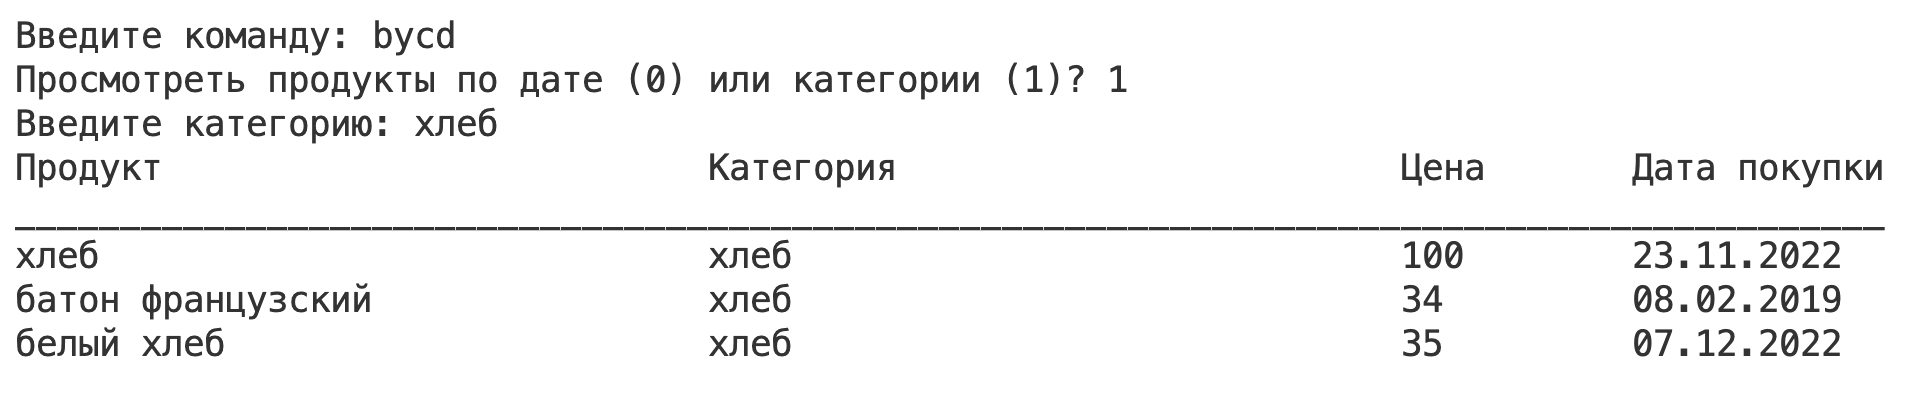
\includegraphics[width=1\linewidth]{Pic16.png}}
\caption{Пример работы команды bycd по категории}
\label{fig26}
\end{figure}

\begin{figure}[H]
\centerline{
\includegraphics[width=1\linewidth]{Pic17.png}}
\caption{Пример работы команды bycd}
\label{fig27}
\end{figure}

\begin{figure}[H]
\centerline{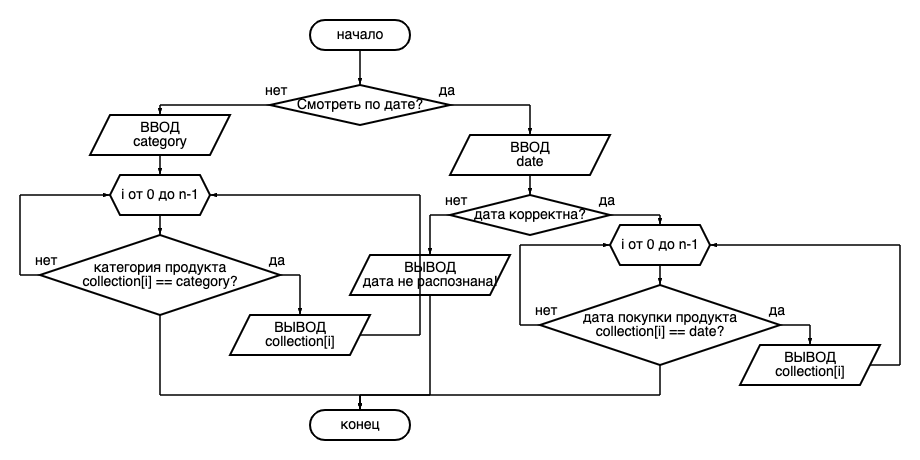
\includegraphics[width=1\linewidth]{diagram3.png}}
\caption{Блок-схема функции bycd()}
\end{figure}

Функция Sort() для сортировки продуктов в коллекции по убыванию / возрастанию (рис. \ref{fig28}). Пользователь выбирает, как хочет сортировать продукты, программа выводит все продукты (рис. \ref{fig29}). Для вывода вызывается ранее описанная функция All().

\begin{figure}[H]
\centerline{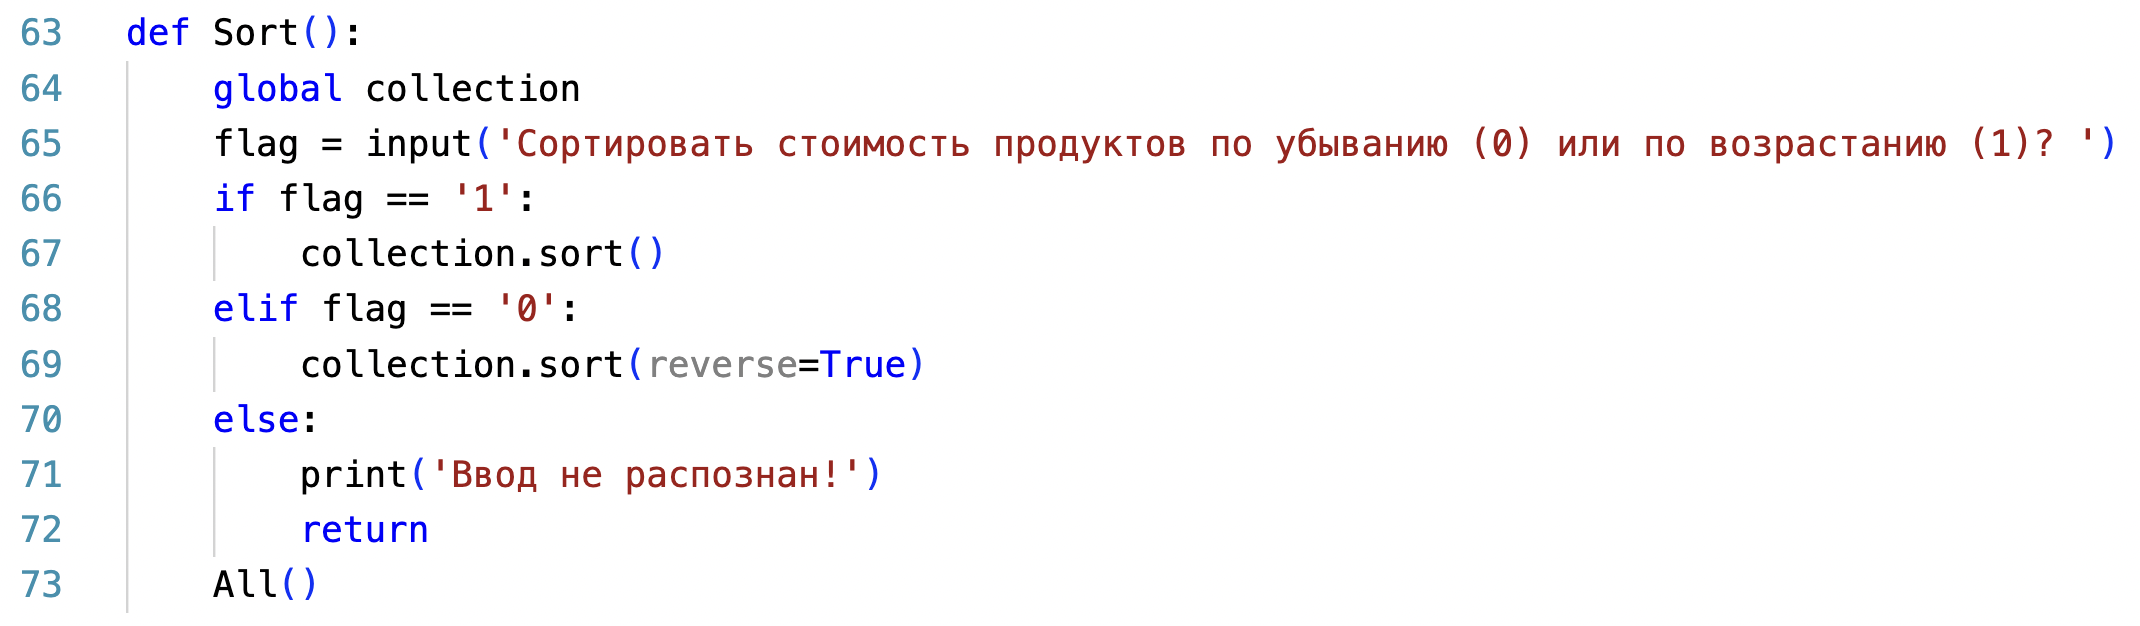
\includegraphics[width=1\linewidth]{Pic18.png}}
\caption{Код функции Sort()}
\label{fig28}
\end{figure}

\begin{figure}[H]
\centerline{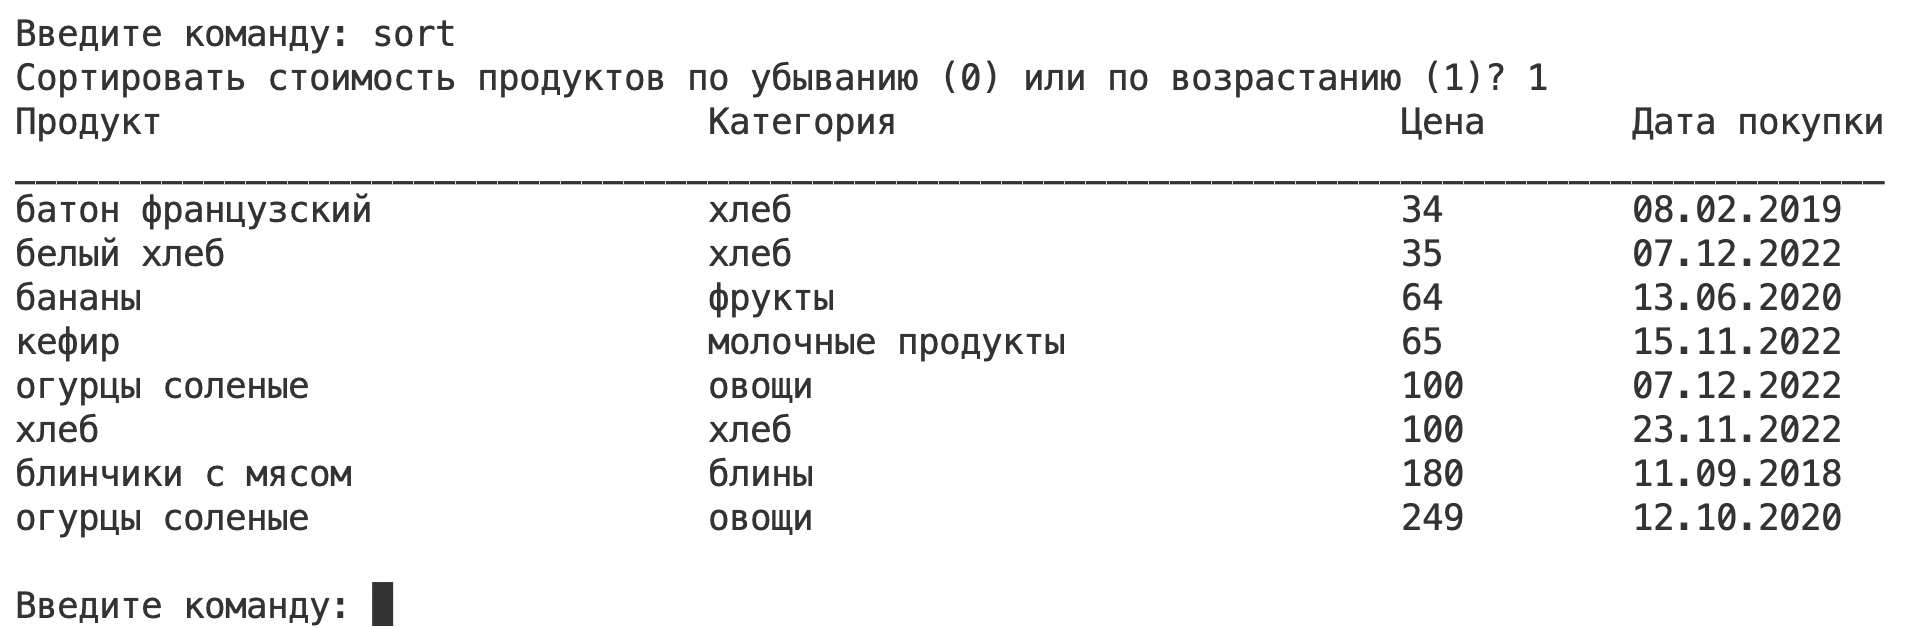
\includegraphics[width=1\linewidth]{Pic19.png}}
\caption{Пример работы команды sort}
\label{fig29}
\end{figure}

Функция Del() для удаления продукта из коллекции (рис. \ref{fig30}). Пользователь вводит номер продукта, который желает удалить из коллекции (рис. \ref{fig31}). Если пользователь ввел существующий номер продукта, то при выводе коллекции его там не окажется (рис. \ref{fig32}).

\begin{figure}[H]
\centerline{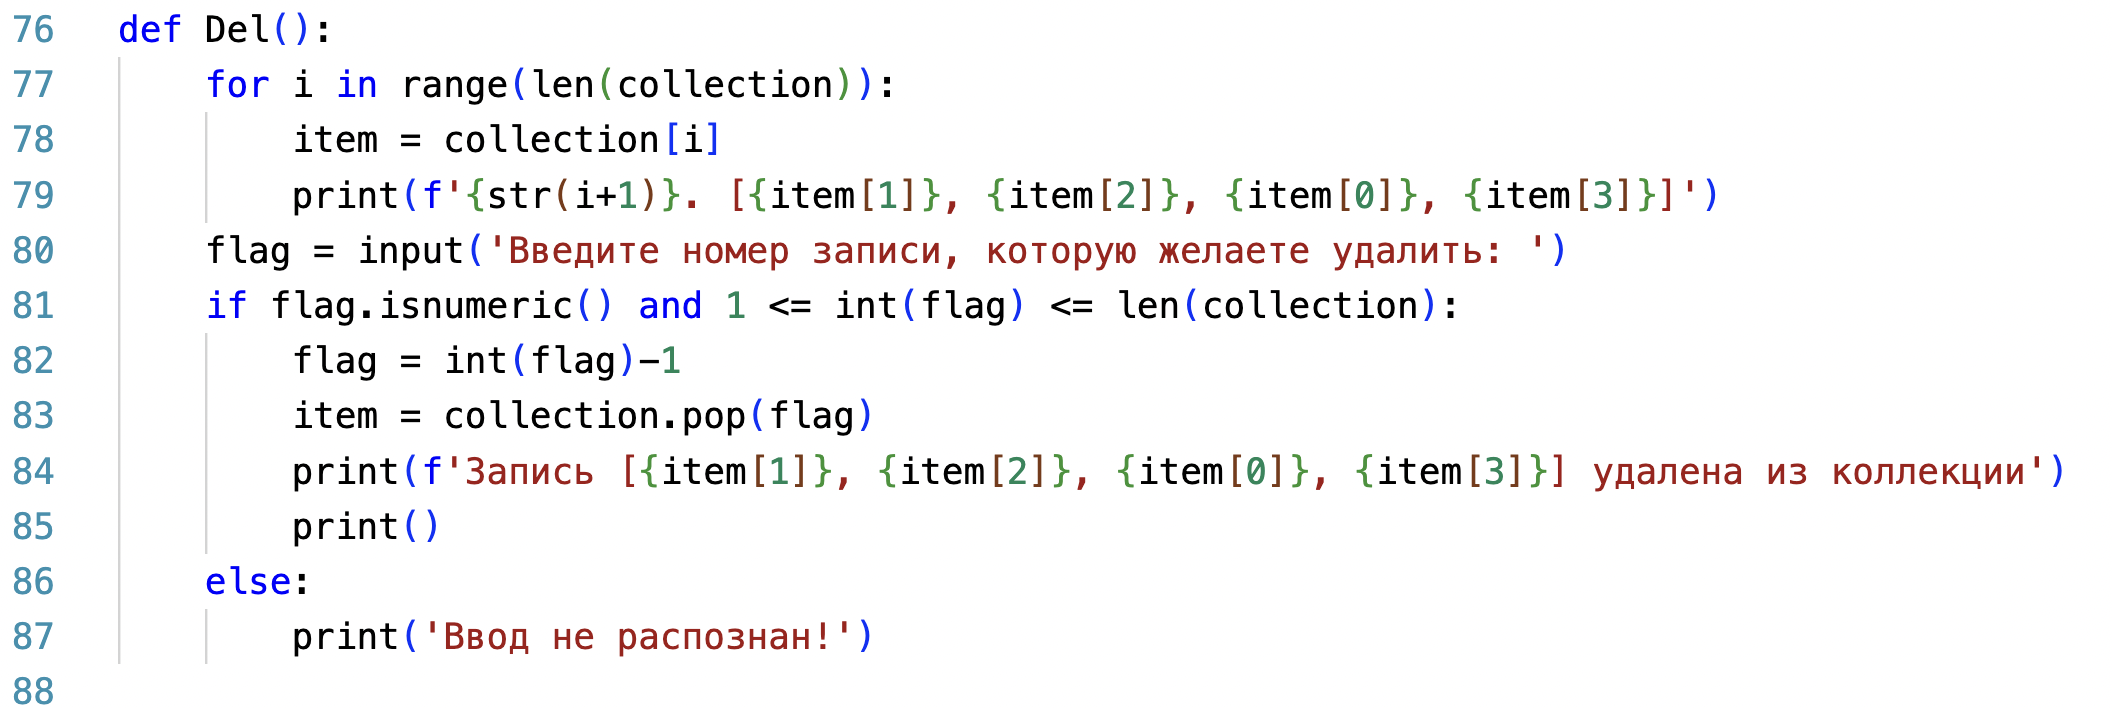
\includegraphics[width=1\linewidth]{Pic20.png}}
\caption{Код функции Del()}
\label{fig30}
\end{figure}

\begin{figure}[H]
\centerline{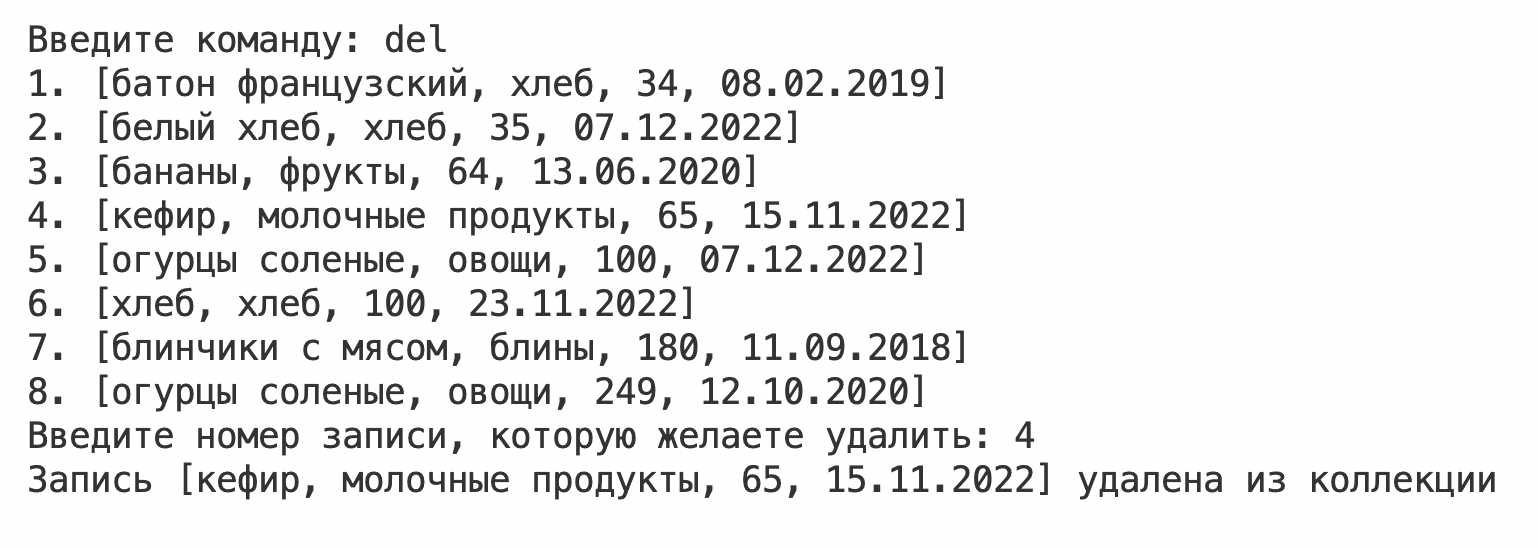
\includegraphics[width=1\linewidth]{Pic21.png}}
\caption{Пример работы команды del}
\label{fig31}
\end{figure}

\begin{figure}[H]
\centerline{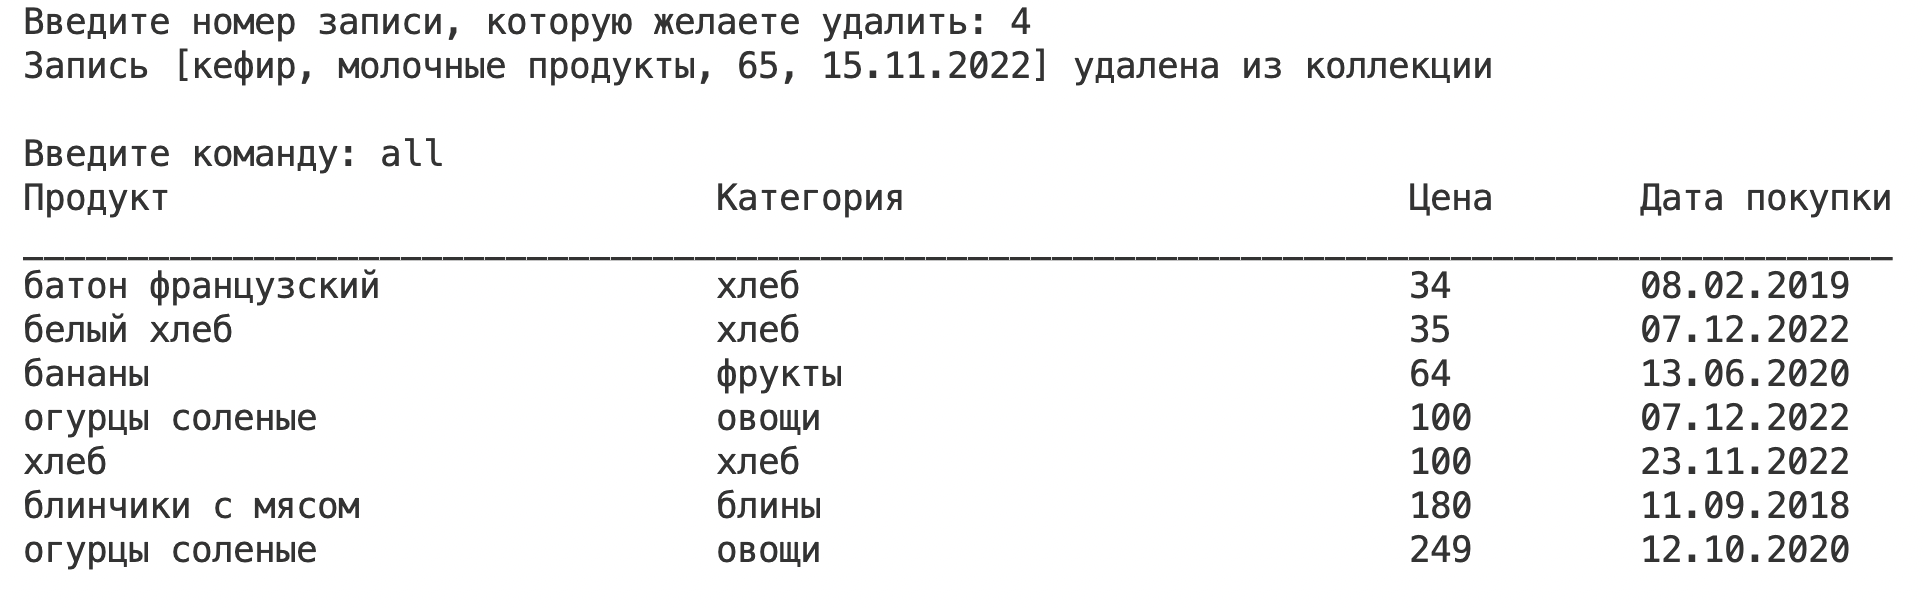
\includegraphics[width=1\linewidth]{Pic22.png}}
\caption{Проверка удаления командой all}
\label{fig32}
\end{figure}

\begin{figure}[H]
\centerline{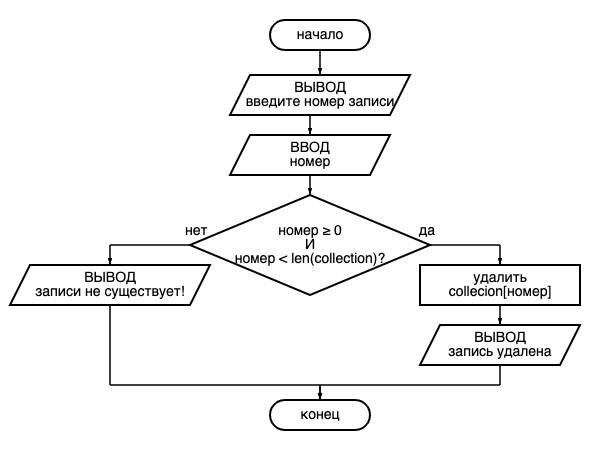
\includegraphics[width=1\linewidth]{diagram4.png}}
\caption{Блок-схема функции Del()}
\end{figure}

Функция save() сохраняет все продукты в коллекции (рис. \ref{fig33}). Файл data.txt, который лежит в директории программы, перезаписывается данными из списка collection. Продукт «белый хлеб», который был добавлен ранее, успешно записался в файл (рис. \ref{fig35})

\begin{figure}[H]
\centerline{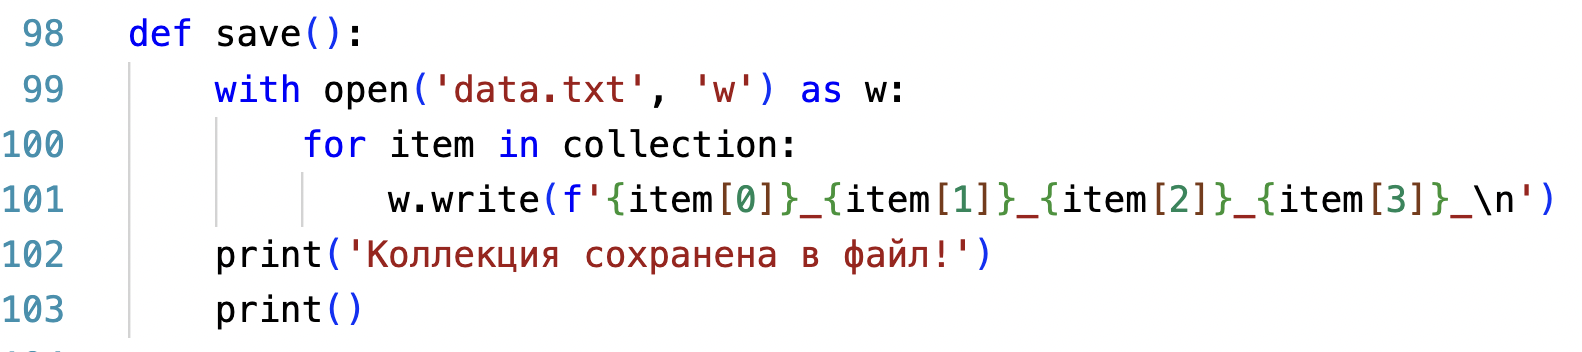
\includegraphics[width=1\linewidth]{Pic23.png}}
\caption{Код функции save()}
\label{fig33}
\end{figure}

\begin{figure}[H]
\centerline{
\includegraphics[width=0.5\linewidth]{Pic24.png}}
\caption{Вывод команды save}
\label{fig34}
\end{figure}

\begin{figure}[H]
\centerline{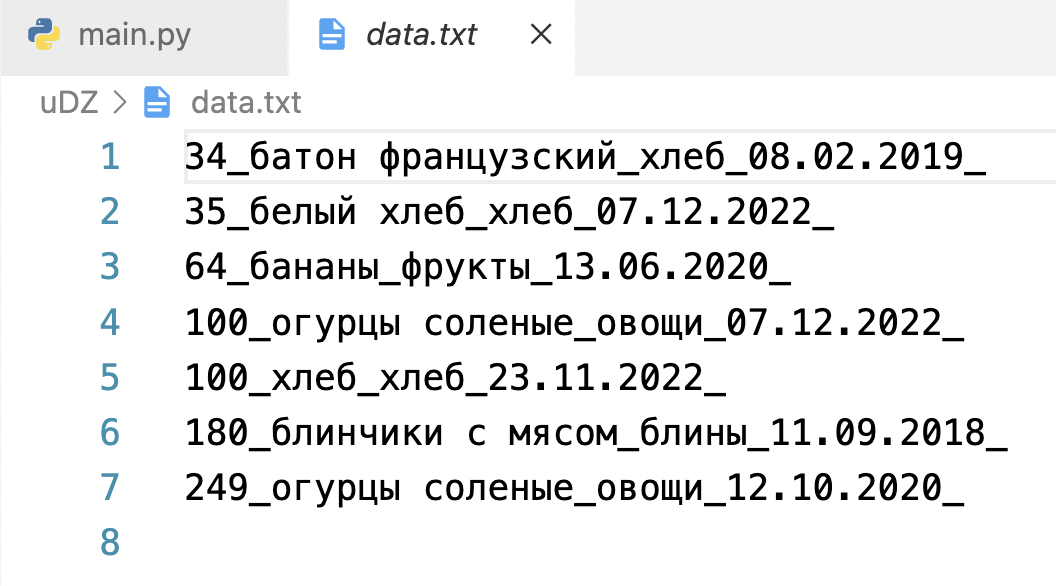
\includegraphics[width=0.6\linewidth]{Pic25.png}}
\caption{Содержимое файла data.txt после выполнения функции}
\label{fig35}
\end{figure}

Когда пользователь закончит работу с программой он может ввести команду exit и программа завершит работу (рис. \ref{fig36})

\begin{figure}[H]
\centerline{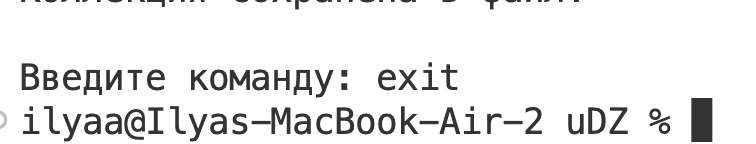
\includegraphics[width=0.4\linewidth]{Pic26.png}}
\caption{Команда exit}
\label{fig36}
\end{figure}

\chapter{Вывод}

Цель работы была достигнута. Было создано программное обеспечение системы обработки данных в виде интерактивного консольного приложения в Python3: «Программа для контроля собственных денежных средств».

Были описаны этапы анализа предметной области и требований. Было описано решение задания с указанием элементов программирования. Были представлены графические материалы, блок-схемы алгоритмов. Была продемонстрирована работа программы.

\end{document}
